\documentclass[landscape]{article}
\usepackage{tikz}
\usepackage[default]{sourcesanspro}
\usepackage[T1]{fontenc}

\pagenumbering{gobble}

\newenvironment{sentencediagram}[3]
    {
        \begin{center}
            {
                \fontfamily{cmr}\selectfont
                #1 \newline
            }

            \footnotesize #2, \textit{#3}
            \LARGE 
    }
    {\end{center}}

\begin{document}

\begin{sentencediagram}{It was a bright cold day in April, and the clocks were striking thirteen.}{George Orwell}{1984}
    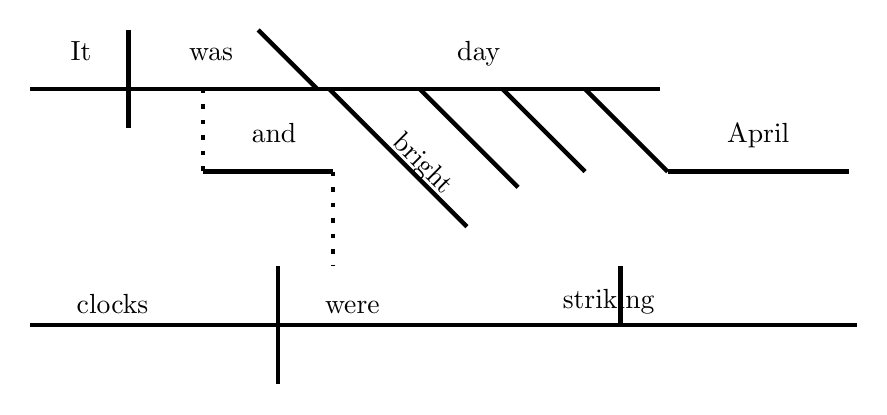
\begin{tikzpicture}
        \draw[ultra thick] (-5, 1.75) -- (3, 1.75);
        \draw[ultra thick] (-3.75, 2.5) -- (-3.75, 1.25);
        \draw[ultra thick] (-2.1, 2.5) -- (-1.35, 1.75);
        \draw[ultra thick] (-1.2, 1.75) -- (-0.3, 0.85)  -- (0.55, 0) node[sloped, above=-0.15cm, pos=0.2]{bright};

        \draw[ultra thick] (-0.05, 1.75) -- (1.2, 0.5);
        \draw[ultra thick] (1, 1.75) -- (2.05, 0.7);
        \draw[ultra thick] (2.05, 1.75) -- (3.1, 0.7);

        \draw[loosely dotted, ultra thick] (-2.8, 1.75) -- (-2.8, 0.7);
        \draw[ultra thick] (-2.8, 0.7) -- (-1.15, 0.7);
        \draw[ultra thick] (3.1, 0.7) -- (5.4, 0.7);
        \draw[loosely dotted, ultra thick] (-1.15, 0.7) -- (-1.15, -0.5);

        \draw[ultra thick] (-5, -1.25) -- (5.5, -1.25)
            node[above, pos=.1]{clocks}
            node[above, pos=.39]{were}
            node[above, pos=.7]{striking};
        \draw[ultra thick] (-1.85, -0.5) -- (-1.85, -2.0);
        \draw[ultra thick] (2.5, -1.25) -- (2.5, -0.5);

        \node at (-4.35, 2.2) {\strut It};
        \node at (-2.7, 2.2) {\strut was};
        \node at (0.7, 2.2) {\strut day};
        \node at (4.25, 1.15) {\strut April};
        \node at (-1.9, 1.15) {\strut and};
        %\node at (-3.75, -0.8) {\strut clocks};
        %\node at (-0.9, -0.8) {\strut were};
        %\node at (1.2, -0.8) {\strut striking};
        %\node at (3.9, -0.8) {\strut thirteen};
    \end{tikzpicture}
\end{sentencediagram}

\end{document}
